\small
\section{引言}
\frame
{
	\frametitle{材料模拟的作用与地位}
\begin{figure}[h!]
\vspace*{-0.18in}
\centering
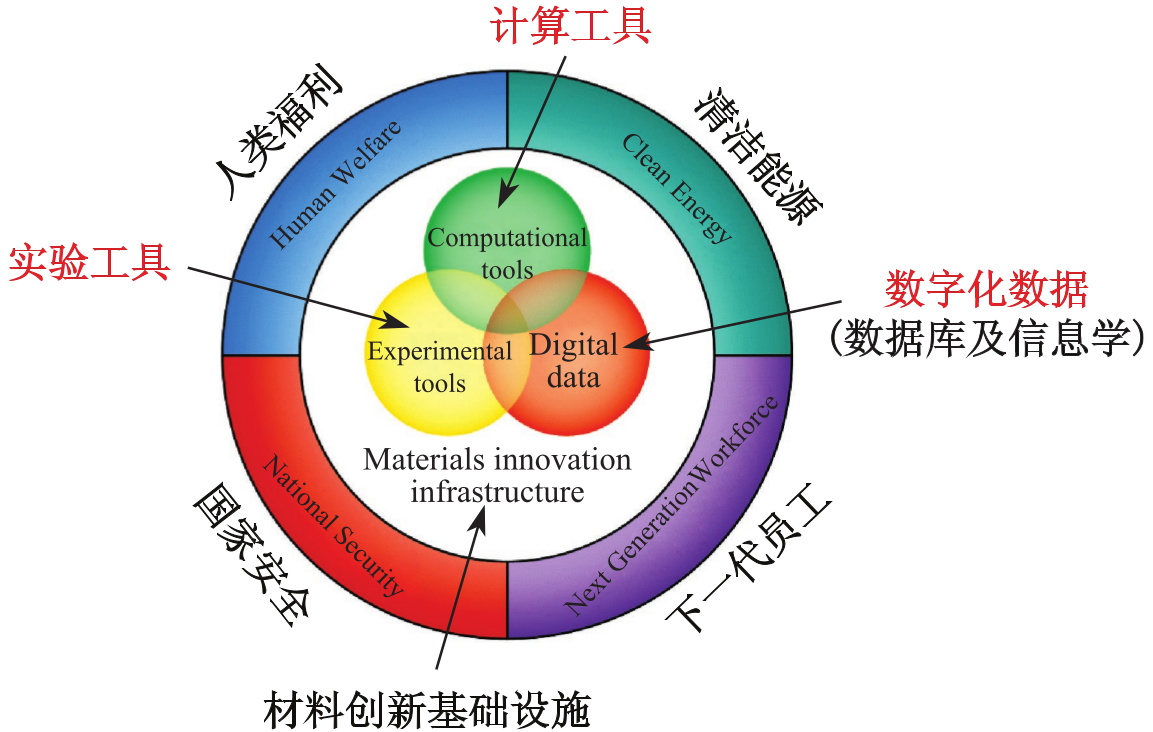
\includegraphics[height=2.55in,width=4.05in]{Figures/MGE.png}
%\caption{\tiny \textrm{Pseudopotential for metallic sodium, based on the empty core model and screened by the Thomas-Fermi dielectric function.}}%(与文献\cite{EPJB33-47_2003}图1对比)
%\caption{\tiny \textrm{Pseudopotential for metallic sodium, based on the empty core model and screened by the Thomas-Fermi dielectric function.}}%(与文献\cite{EPJB33-47_2003}图1对比)
\label{MGE}
\end{figure}
}

\frame
{
	\frametitle{材料模拟的基本思想和方法}
\begin{figure}[h!]
\vspace*{-0.25in}
\centering
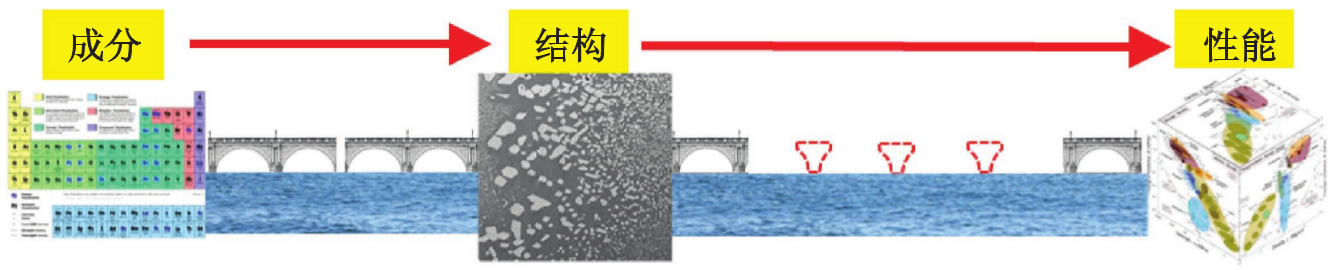
\includegraphics[height=0.80in,width=4.05in]{Figures/MGE-2.png}
%\caption{\tiny \textrm{Pseudopotential for metallic sodium, based on the empty core model and screened by the Thomas-Fermi dielectric function.}}%(与文献\cite{EPJB33-47_2003}图1对比)
\vskip 0.05pt
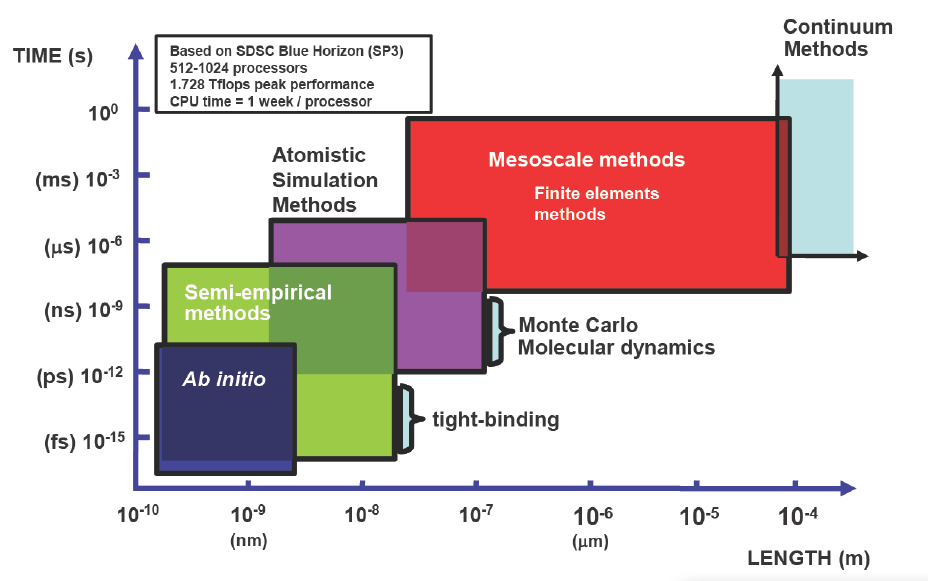
\includegraphics[height=2.20in,width=3.45in]{Figures/Multi-Scale-6.png}
%\caption{\tiny \textrm{Pseudopotential for metallic sodium, based on the empty core model and screened by the Thomas-Fermi dielectric function.}}%(与文献\cite{EPJB33-47_2003}图1对比)
\label{Multi-Scale}
\end{figure}
}

\frame
{
	\frametitle{\rm{I~Have~A~Dream}}
\begin{figure}[h!]
\vspace*{-0.18in}
\centering
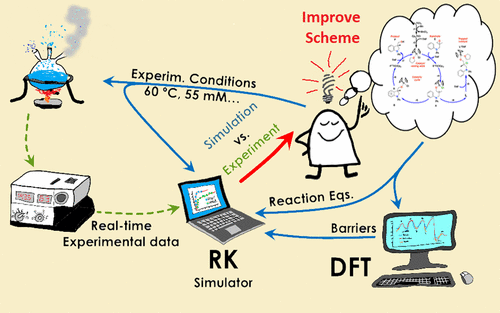
\includegraphics[height=2.55in,width=4.05in]{Figures/Schematic_Material-Design.png}
%\caption{\tiny \textrm{Pseudopotential for metallic sodium, based on the empty core model and screened by the Thomas-Fermi dielectric function.}}%(与文献\cite{EPJB33-47_2003}图1对比)
%\caption{\tiny \textrm{Pseudopotential for metallic sodium, based on the empty core model and screened by the Thomas-Fermi dielectric function.}}%(与文献\cite{EPJB33-47_2003}图1对比)
\label{Schematic_Material-Design}
\end{figure}
}

\section{量子力学基础}
\frame
{
	\frametitle{量子力学的奠基人}
\begin{figure}[h!]
\centering
%\vspace{-25.5pt}
%\hspace*{-15.5pt}
%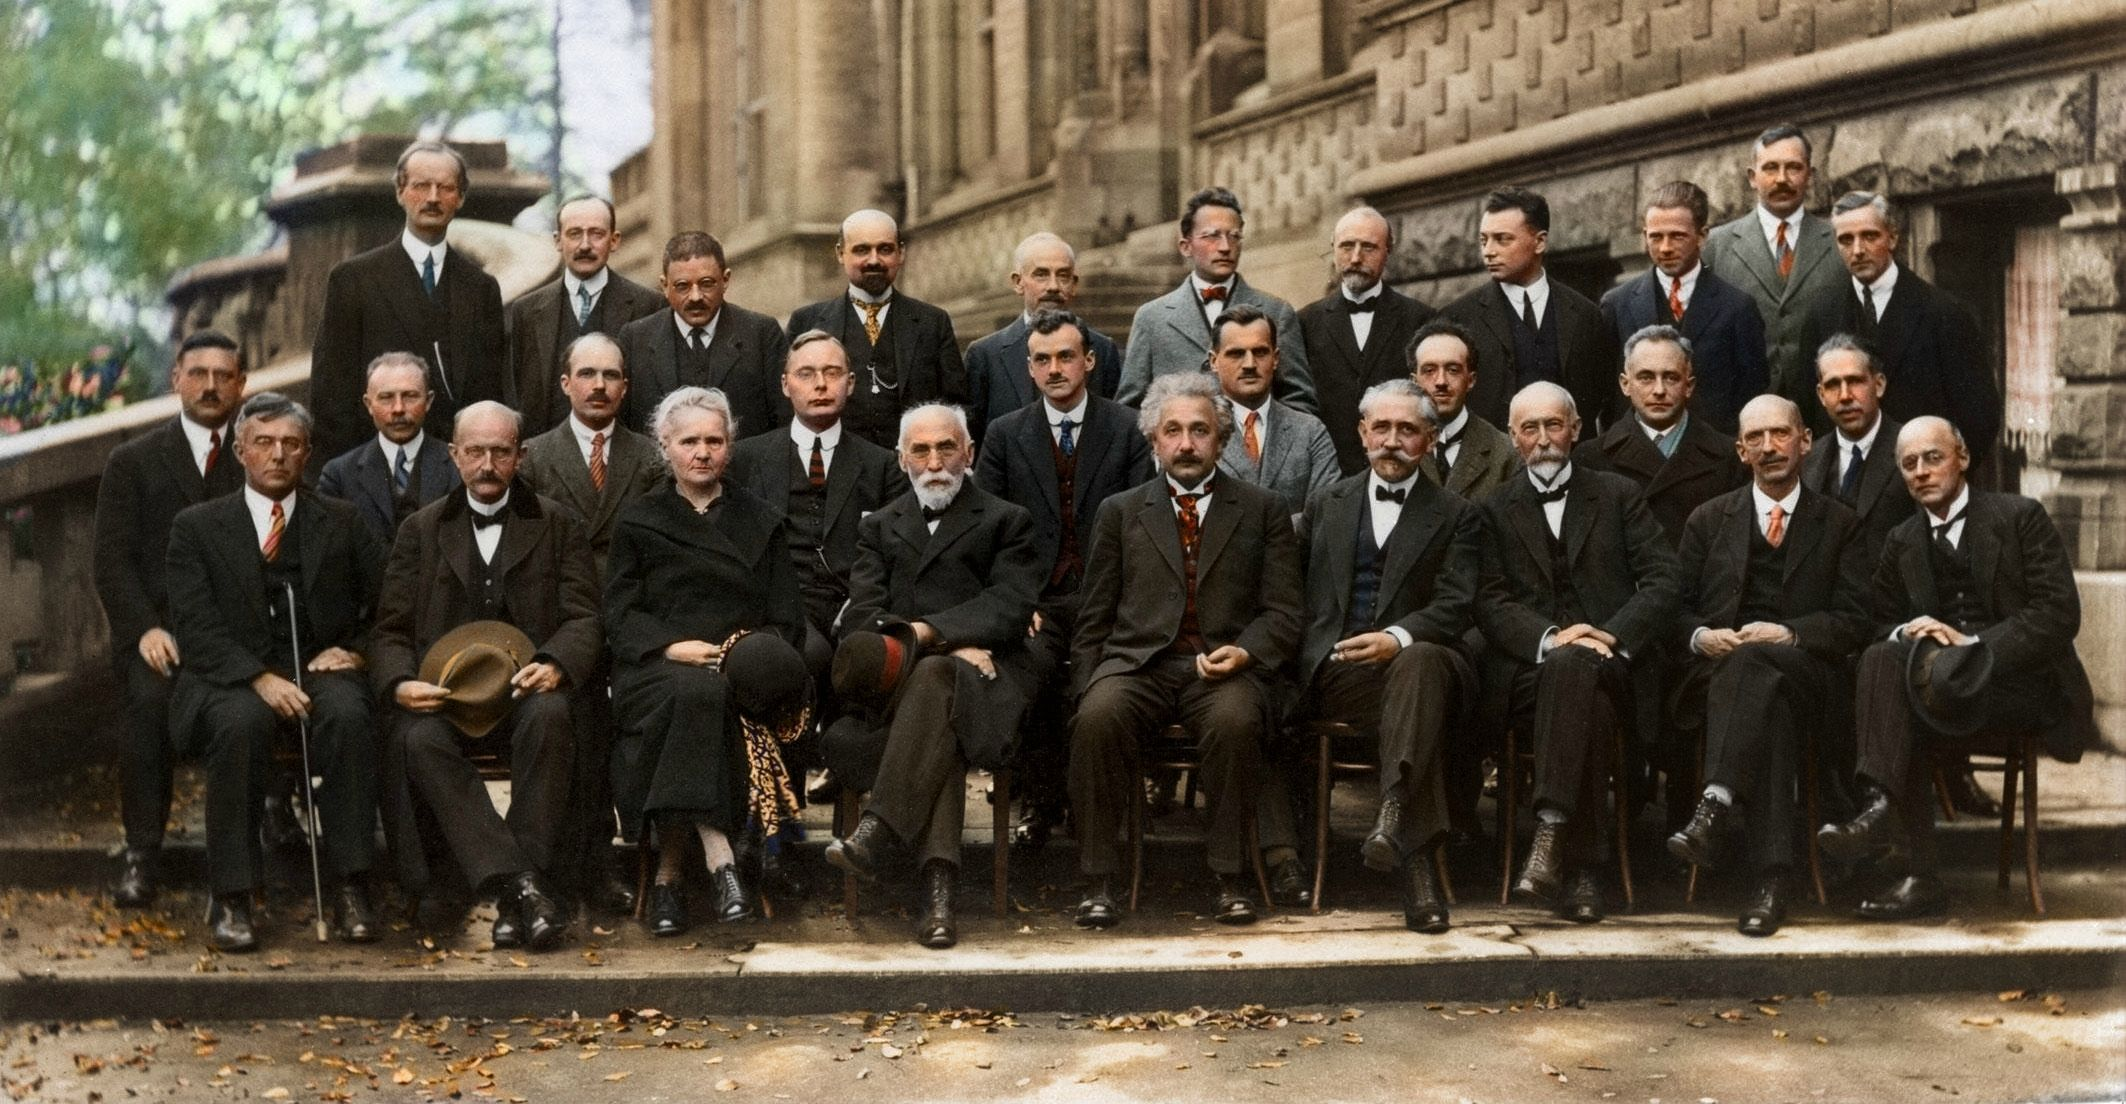
\includegraphics[height=0.57\textwidth,width=1.1\textwidth,viewport=0 0 2150 1050,clip]{Figures/Solvay_Conference-5-fine.jpg}
\vspace{-14.5pt}
\hspace*{-15.5pt}
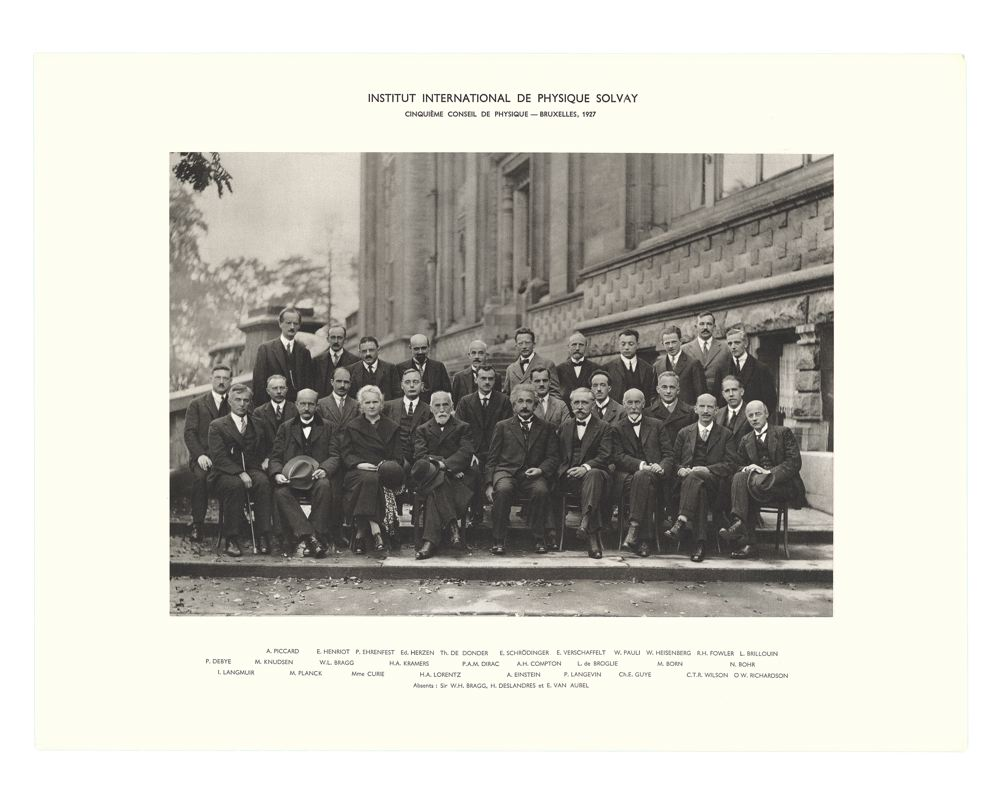
\includegraphics[height=0.50\textwidth,width=0.70\textwidth,viewport=150 105 850 710,clip]{Figures/Solvay_Conference-5.jpg}
\caption{\fontsize{7.5pt}{6.2pt}\selectfont{\textrm{The Fifth Solvay International Conference, Brussels, Belgium, Oct. 1927}}}
\label{Solvay Conference-5-fine}
\end{figure}
\vspace{-11.5pt}
\fontsize{4.1pt}{3.9pt}\selectfont{\textrm{\textcolor{blue}{前排左起}:~I.Langmuir(\textcolor{blue}{朗缪尔}) M.Planck(\textcolor{blue}{普朗克}) Marie Curie(\textcolor{blue}{居里夫人}) H.Lorentz(\textcolor{blue}{洛仑兹}) A.Einstein(\textcolor{blue}{爱因斯坦}) P.Langevin(\textcolor{blue}{朗之万}) Ch.E.Guye(\textcolor{blue}{古伊}) C.T.R.Wilson(\textcolor{blue}{威尔逊}) O.W.Richardson(\textcolor{blue}{理查森})\\
\textcolor{blue}{中排左起}:~P.Debye(\textcolor{blue}{德拜}) M.Knudsen(\textcolor{blue}{克努森}) W.L.Bragg(\textcolor{blue}{布拉格}) H.A.Kramers(\textcolor{blue}{克莱默}) P.A.M.Dirac(\textcolor{blue}{狄拉克}) A.H.Compton(\textcolor{blue}{康普顿}) L.de Broglie(\textcolor{blue}{德布罗意}) M.Born(\textcolor{blue}{玻恩}) N.Bohr(\textcolor{blue}{玻尔})\\
\textcolor{blue}{后排左起}:~A.Piccard(\textcolor{blue}{皮卡尔德}) E.Henriot(\textcolor{blue}{亨利厄特}) P.Ehrenfest(\textcolor{blue}{埃伦费斯特}) Ed.Herzen(\textcolor{blue}{赫尔岑}) Th.de Donder(\textcolor{blue}{德唐德}) E.Schr\"odinger(\textcolor{blue}{薛定谔}) E.Verschaffelt(\textcolor{blue}{费尔夏费尔特}) W.Pauli(\textcolor{blue}{泡利}) W.Heisenberg(\textcolor{blue}{海森堡}) R.H.Fowler(\textcolor{blue}{富勒}) L.Brillouin(\textcolor{blue}{布里渊})}}
}
%------------------------------------------------------------------------Reference----------------------------------------------------------------------------------------------
\frame
{
	\frametitle{黑体辐射与能量量子化}
	\textrm{1900}年,为了解释黑体辐射\textrm{(black-body radiation)}的能量密度与辐射频率的关系,\textrm{M.~Planck}引入\textcolor{red}{能量量子化}的假设,利用统计物理推导出与实验符合得非常好的黑体辐射\textrm{Planck~}公式:~
	\begin{displaymath}
		\rho_{\nu}\mathrm{d}{\nu}=\dfrac{8{\pi}h{\nu}^3}{C^3}\bigg(\dfrac1{\mathrm{e}^{h\nu/kT}-1}\bigg)\mathrm{d}\nu
	\end{displaymath}
\begin{figure}[h!]
\centering
\vspace{-10.5pt}
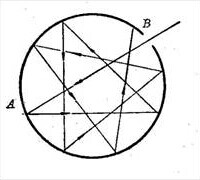
\includegraphics[height=1.45in,width=1.45in,viewport=0 0 136 136,clip]{Figures/Black_box.jpg}
\hskip 1pt
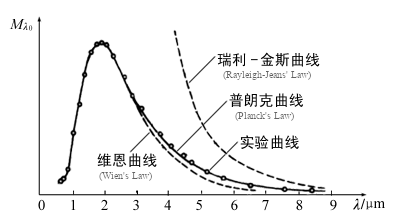
\includegraphics[height=1.32in,width=2.25in,viewport=0 0 390 215,clip]{Figures/Black_box_curve.png}
\caption{\textrm{The black-body radiation and the curve}}
\label{Black_box}
\end{figure}
}

\frame
{
	\frametitle{几何原本:~公理体系的源头}
\begin{figure}[h!]
\centering
\vspace{-13pt}
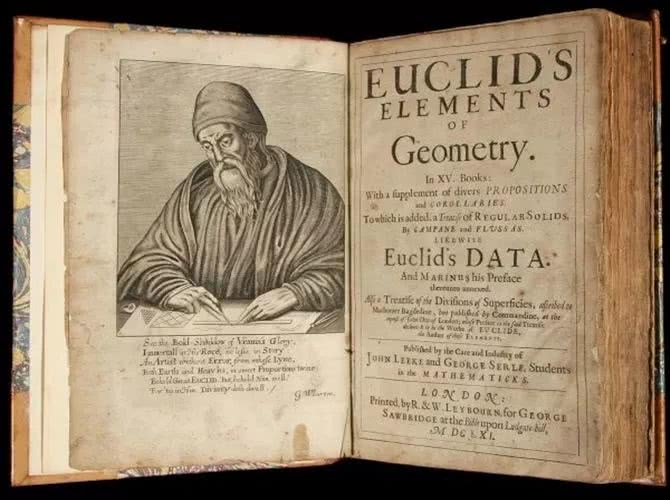
\includegraphics[height=0.38\textwidth,width=0.65\textwidth,viewport=0 0 680 500,clip]{Figures/Element_Geometry_1.jpg}\\
\vspace{1pt}
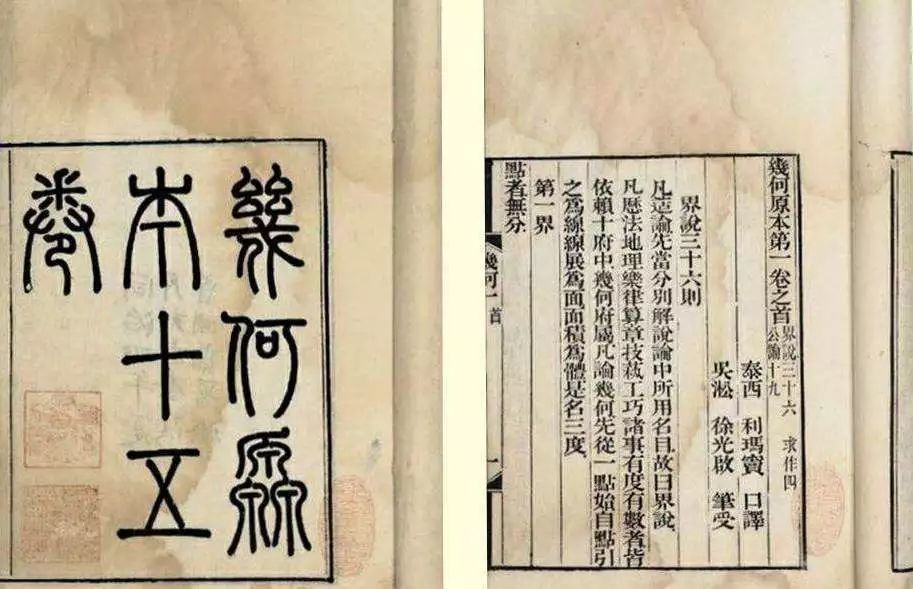
\includegraphics[height=0.36\textwidth,width=0.65\textwidth,viewport=0 0 810 500,clip]{Figures/Element_Geometry_2.jpg}
%\caption{\textrm{ABINIT}的Si.in}
\label{Element_Geometru}
\end{figure}
}

\frame
{
	\frametitle{\textcolor{red}{公理体系}:~现代科学的逻辑起点}
\begin{figure}[h!]
\centering
\vspace{-10.5pt}
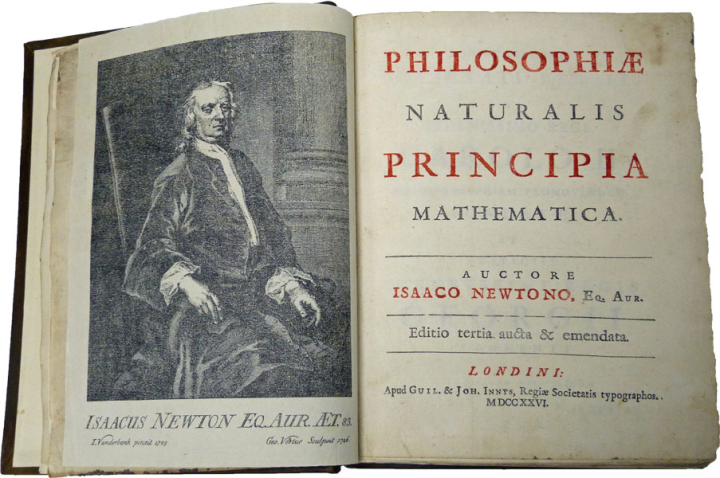
\includegraphics[height=0.68\textwidth,width=1.0\textwidth,viewport=0 0 770 500,clip]{Figures/Philp_Nature_Mach-2.png}
%\caption{\textrm{ABINIT}的Si.in}
\label{Philp_Nature}
\end{figure}
}

\frame
{
	\frametitle{\textrm{\small Newtonian, Lagrangian and Hamiltonian Mechanics}}
	\begin{itemize}
   		\setlength{\itemsep}{10pt}
		\item \textrm{\textcolor{blue}{Newtonian~Mechanics}}\\
		牛顿运动定律体系是以力、加速度、动量这些矢量为基本量来描述力学系统在欧氏空间的运动~(用几何方程表述约束)
	\item \textrm{\textcolor{blue}{Lagrangian~Mechanics}}\\
		拉格朗日力学是关于研究对象在其对应的约束系统下的运动形式,大大压缩牛顿方程描述需要的约束个数。不需要在另外设未知数目
	\item \textrm{\textcolor{blue}{Hamiltonian~Mechanics}}\\
		哈密度力学由拉格朗日力学演变而来,把位置和动量彻底分开,成为两种独立变量,由此诞生相空间。把广义动量和广义坐标放在等同的位置上(正则配对,方程降阶)
		\vskip 6pt
		拉格朗日力学和哈密顿力学的基本量是系统的能量等标量,通过变分原理建立系统的动力学方程,所以拉格朗日力学和哈密顿力学合称\textcolor{magenta}{分析力学}
	\end{itemize}
}

\frame
{
	\frametitle{量子力学基本假设(\textcolor{red}{公理体系})}
	\begin{itemize}
		\item 全同粒子假设\\
			\textcolor{blue}{全同粒子组成的体系中,两个全同粒子相互调换不改变体系的状态}\\ 
			全同粒子是指\textcolor{red}{内禀性质完全相同的一类微观粒子}:\\例如,所有的电子是全同粒子 
		\item 波函数假设\\
			\textcolor{blue}{微观体系的运动状态可由波函数$\Psi$完全描述,波函数包含体系的所有性质}\\
			波函数$\Psi$一般要求满足\textcolor{red}{连续}、\textcolor{red}{有限}和\textcolor{red}{单值}三个条件
		\item 态叠加原理\\
			如果$\Psi_1$是体系的一个本征态,对应的本征值为$A_1$,$\Psi_2$也是体系的一个本征态,对应的本征值为$A_2$,则\textcolor{blue}{$$\Psi=C_1\Psi_1+C_2\Psi_2$$}\textcolor{red}{也是体系一个可能的存在状态}
	\end{itemize}
}

\frame
{
	\frametitle{\textrm{Schr\"odinger's cat}}
\begin{figure}[h!]
\centering
\vspace{-10.5pt}
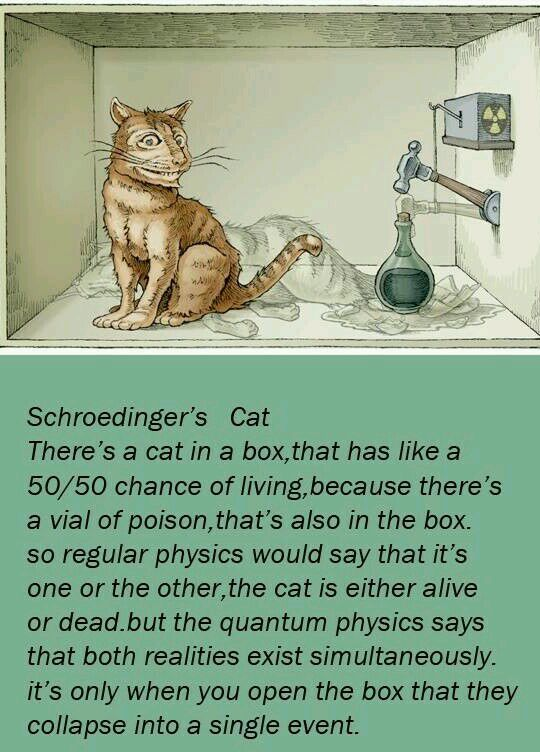
\includegraphics[height=0.70\textwidth,width=0.7\textwidth,viewport=0 0 760 750,clip]{Figures/Schrodinger-cat.jpg}
%\caption{\textrm{ABINIT}的Si.in}
\label{Schrodinger-cat}
\end{figure}
}

\frame
{
	\frametitle{叠加态的数学表示:~矩阵}
\begin{figure}[h!]
\centering
\vspace{-1.5pt}
\hspace*{-0.12in}
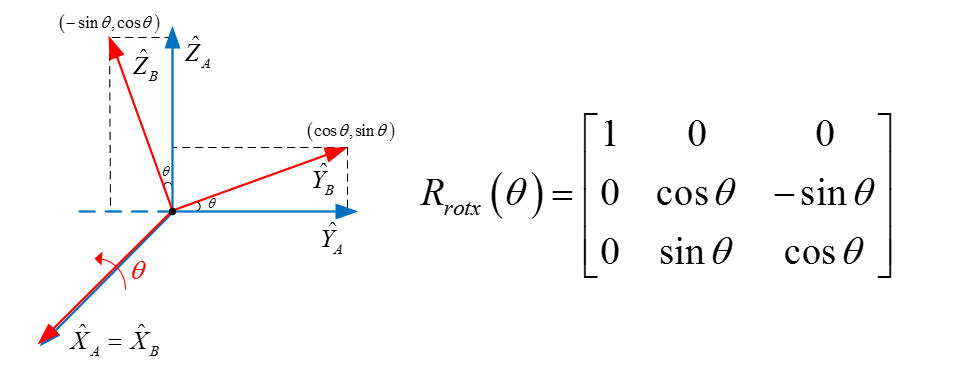
\includegraphics[height=0.48\textwidth,width=1.05\textwidth]{Figures/Matrix_Rotation.png}
%\caption{\textrm{ABINIT}的Si.in}
\label{Matrix-Rotation}
\end{figure}
}

\frame
{
	\frametitle{量子力学基本假设(续)}
	\begin{itemize}
		\item 力学量算符假设\\
			\textcolor{blue}{经典力学中的物理量对应到量子力学中,要用线性\textrm{Hermite~}算符表示}(\textcolor{red}{\textrm{Hermite~}算符的本征函数构成完备空间})\\
			如动量算符 
			$$\hat{\mathbf{p}}=-\mathrm{i}\hbar\nabla$$
			位置算符$$\hat{\mathbf r}=r$$
			力学量算符之间有确定的对易关系(\textcolor{brown}{量子条件})
			$$[\hat{\mathbf F},\hat{\mathbf G}]=\hat{\mathbf F}\hat{\mathbf G}-\hat{\mathbf G}\hat{\mathbf F}$$ 
			
		\item 微观体系的运动状态\textcolor{blue}{波函数随时间变化的规律}:\\\textcolor{red}{遵从\textrm{Schr\"odinger}方程}
			$$\mathrm{i}\hbar\dfrac{\mathrm{d}}{\mathrm{d}t}|\Psi\rangle=\hat{\mathbf H}|\Psi\rangle$$
	\end{itemize}
}

\frame
{
	\frametitle{驻波方程与势阱}
\begin{figure}[h!]
\centering
\vspace{-12.5pt}
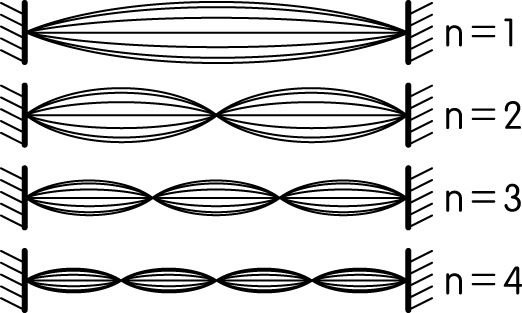
\includegraphics[height=0.32\textwidth,width=0.7\textwidth,viewport=0 0 125 75,clip]{Figures/Standing_wave.jpeg}
\vskip 2pt
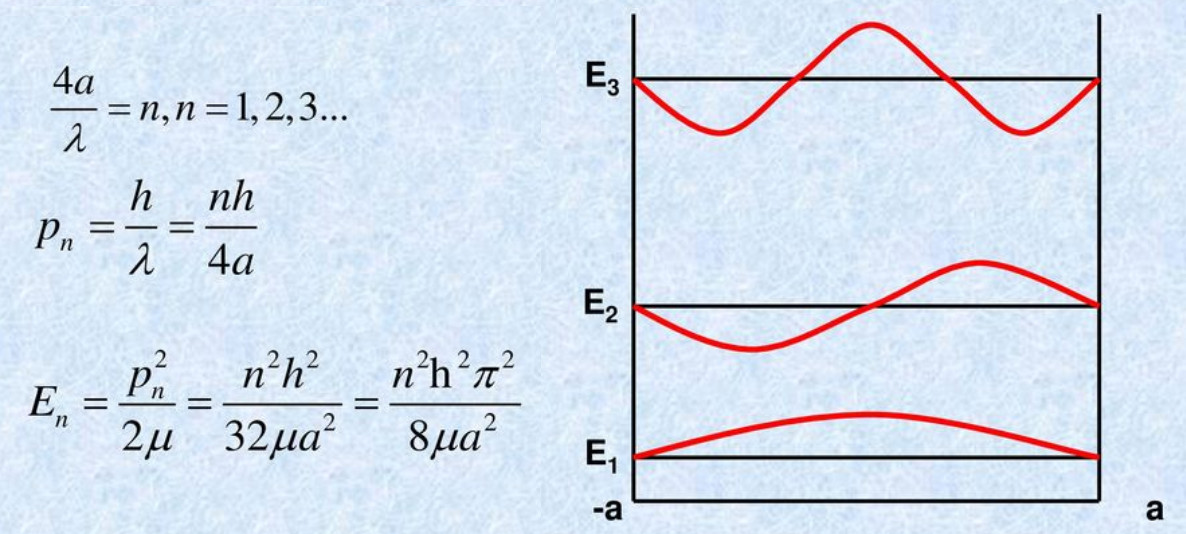
\includegraphics[height=0.40\textwidth,width=0.9\textwidth,viewport=0 0 1200 550,clip]{Figures/Standing_wave-energy.jpg}
%\caption{\textrm{ABINIT}的Si.in}
\label{Standing_Wave_1}
\end{figure}
}

\frame
{
	\frametitle{驻波方程与势阱}
\begin{figure}[h!]
\centering
\vspace{-5.5pt}
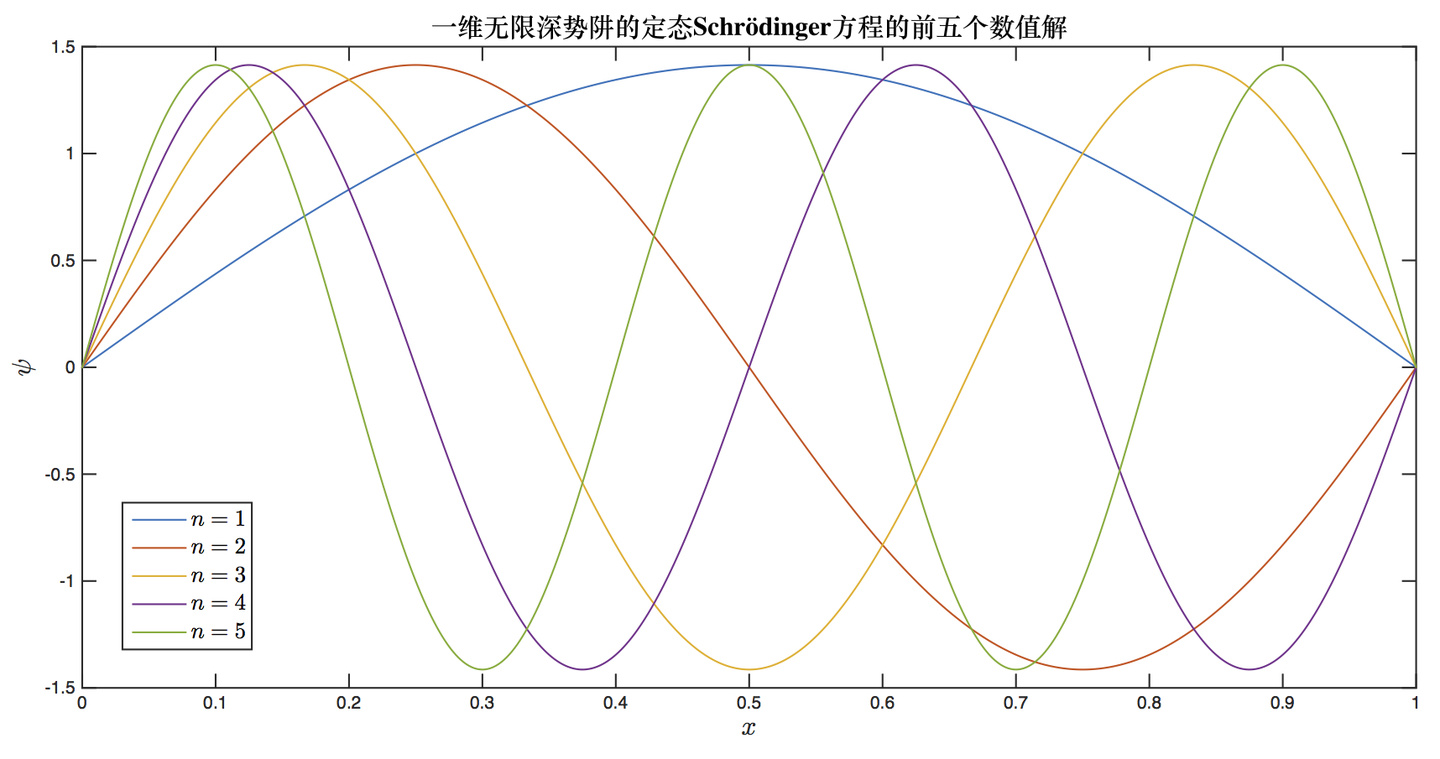
\includegraphics[height=0.55\textwidth,width=1.0\textwidth,viewport=0 0 720 400,clip]{Figures/Standing_wave-energy_1-5.jpg}
%\caption{\textrm{ABINIT}的Si.in}
\label{Standing_Wave_2}
\end{figure}
}

\frame
{
	\frametitle{驻波方程与势阱}
\begin{figure}[h!]
\centering
\vspace{-0.5pt}
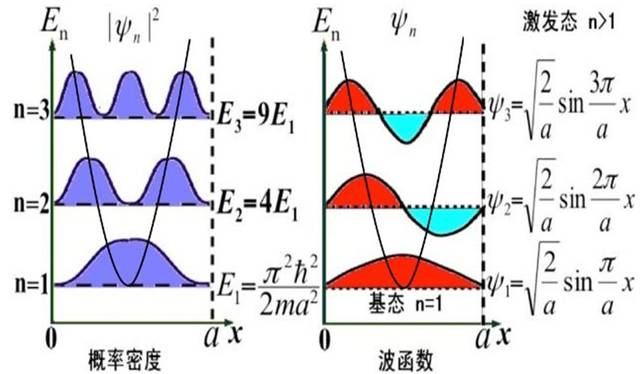
\includegraphics[height=0.46\textwidth,width=1.0\textwidth,viewport=0 0 650 390,clip]{Figures/Standing_wave_Energy.jpeg}
%\caption{\textrm{ABINIT}的Si.in}
\label{Standing_Wave_2}
\end{figure}
}

\frame
{
	\frametitle{原子的驻波方程}
\begin{figure}[h!]
	\vspace{-10.5pt}
\centering
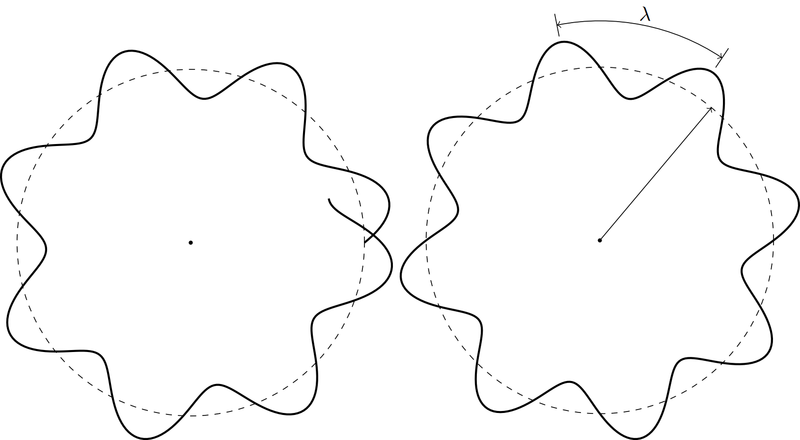
\includegraphics[height=0.38\textwidth,width=0.74\textwidth,viewport=0 0 840 440,clip]{Figures/Standing_wave-atom.png}
\vskip 2pt
\animategraphics[autoplay, loop, height=1.3in]{1}{Figures/Standing_wave_circle_}{1}{25}
\label{Atomic_Standing_wave}
\end{figure}
}

\frame
{
	\frametitle{\textrm{Schr\"odinger}~方程}
\begin{figure}[h!]
\centering
%
\vspace{-10.5pt}
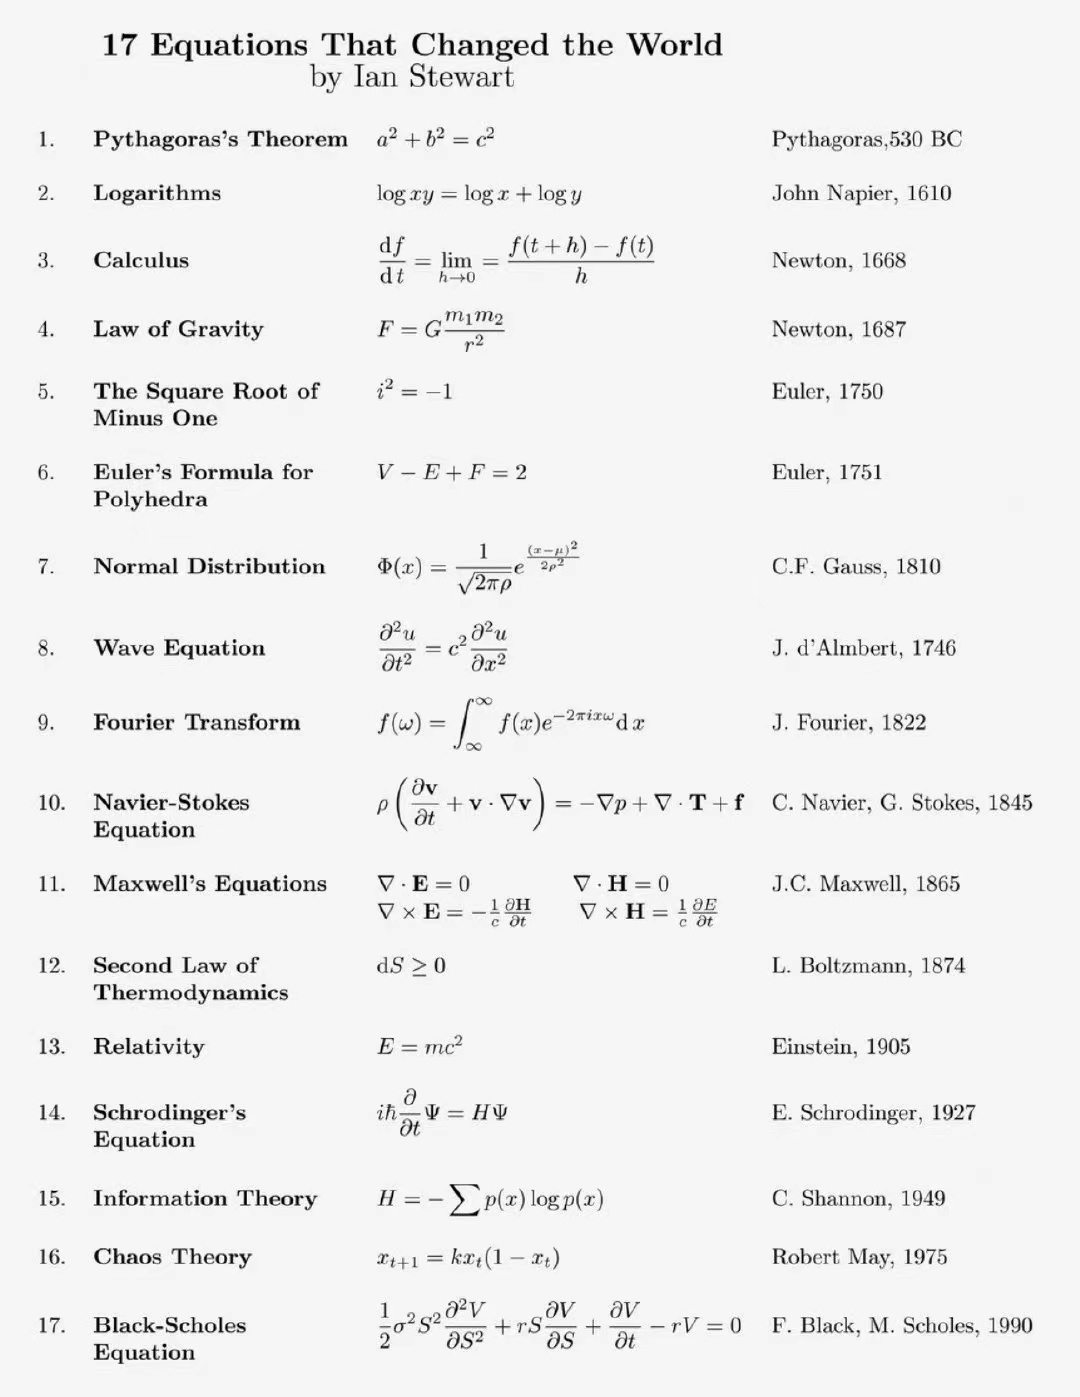
\includegraphics[height=0.72\textwidth,width=0.58\textwidth,viewport=0 0 1050 1400,clip]{Figures/Great_Equation.jpg}
\label{Great_Equation}
\end{figure}
}

\frame
{
%	\frametitle{\textrm{DFT-SCF}}
\begin{figure}[h!]
\vspace*{-0.25in}
\centering
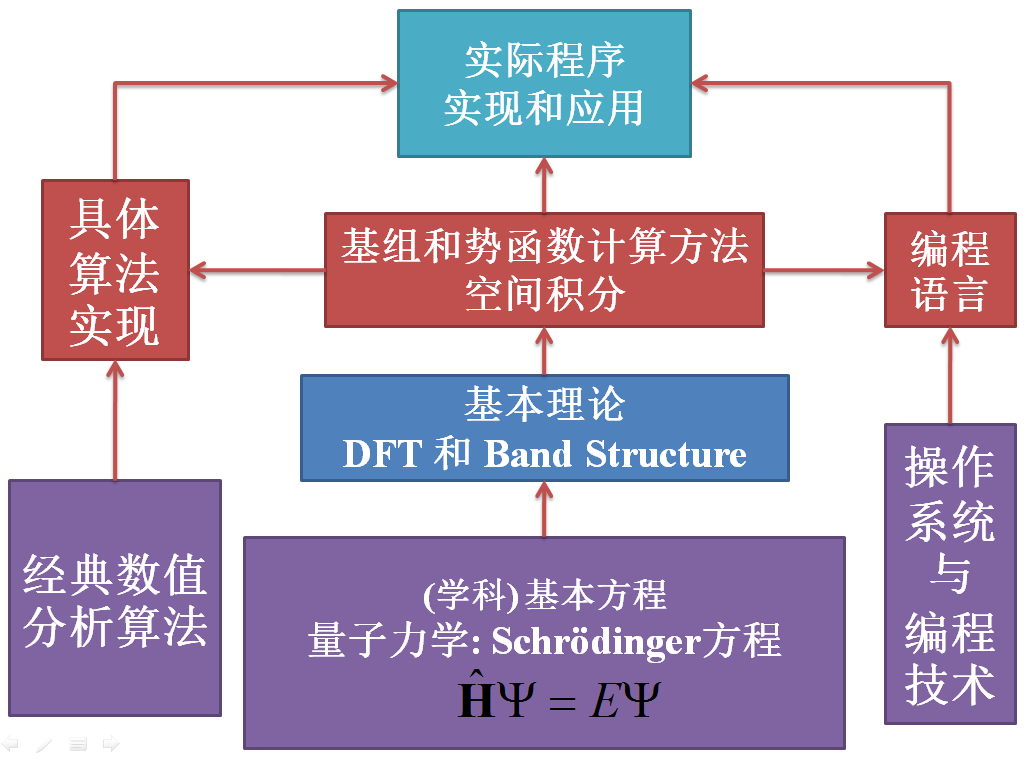
\includegraphics[height=2.80in,width=4.95in,viewport=5 3 1250 780,clip]{Figures/Method_Procedure.png}
%\caption{\tiny \textrm{Pseudopotential for metallic sodium, based on the empty core model and screened by the Thomas-Fermi dielectric function.}}%(与文献\cite{EPJB33-47_2003}图1对比)
\label{Method-Procedure}
\end{figure}
}

%-----------------------------------------------------------------------------
